\documentclass[UTF8,11pt,a4paper]{ctexart}
\usepackage[margin=22mm]{geometry}
\usepackage{amsmath,amssymb,mathtools}
\usepackage{tikz}
\usetikzlibrary{angles,quotes}
\usepackage{hyperref}
\hypersetup{colorlinks=true,linkcolor=blue}
\newcommand{\V}[1]{\overrightarrow{#1}}
\title{一道向量最值题，藏着多少种解法？\\ \large VIDEO-002 数学解析母稿}
\author{Self Media Lab}
\date{v0.1 \quad 2026-11-12}
\begin{document}
\maketitle
\section*{题目（自行重新排版）}
在平面四边形 $ABCD$ 中，已知
\[
AB=2,\quad AC=2\sqrt3,\quad AC\perp AB,\quad \angle ADC=\frac{2\pi}{3}.
\]
求 $\V{AD}\cdot\V{AB}$ 的最小值。
选项：A.\ $-\sqrt3$；B.\ $-2\sqrt3$；C.\ $-4$；D.\ $-2$。
\[
\boxed{\min\bigl(\V{AD}\cdot\V{AB}\bigr)=-2\quad\text{（选 D）}}
\]
\section*{原创 TikZ 示意：等号构型}
\begin{center}
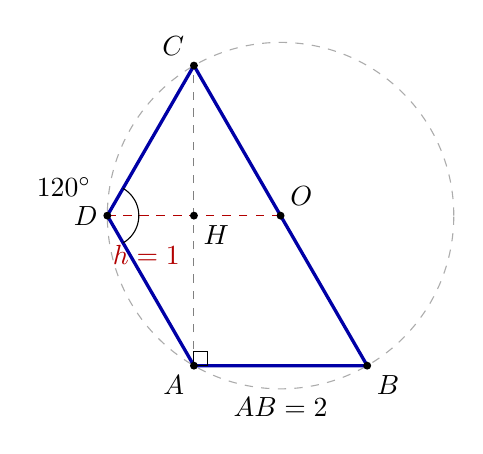
\begin{tikzpicture}[scale=1.1]
\coordinate (A) at (0,0);
\coordinate (B) at (2,0);
\coordinate (C) at (0,3.464101615);
\coordinate (D) at (-1,1.732050808);
\coordinate (O) at (1,1.732050808);
\coordinate (H) at (0,1.732050808);
\draw[gray!65,dashed] (O) circle (2);
\draw[very thick,blue!65!black] (A)--(B)--(C)--(D)--cycle;
\draw[black!50,dashed] (A)--(C);
\draw[red!70!black,dashed] (D)--(H);
\draw[red!70!black,dashed] (O)--(D);
\draw (0,0) rectangle (.16,.16);
\foreach \P/\pos in {A/below left,B/below right,C/above left,D/left,O/above right,H/below right}
 {\fill (\P) circle (1.3pt) node[\pos] {$\P$};}
\node at (1,-.48) {$AB=2$};
\node[red!70!black] at (-.55,1.28) {$h=1$};
\pic[draw,angle radius=.40cm]{angle=A--D--C};
\node at (-1.50,2.06) {$120^\circ$};
\end{tikzpicture}
\end{center}

\section{解法一：余弦定理 + 面积 + 基本不等式（正片主讲）}
设 $AD=a,CD=b$。因 $\angle ADC=120^\circ$，余弦定理给出
\[
AC^2=a^2+b^2-2ab\cos120^\circ=a^2+b^2+ab=12.
\]
由 $a^2+b^2\ge 2ab$ 得
\[
12\ge 3ab,\qquad \boxed{ab\le4}.
\]
令 $h$ 为点 $D$ 到直线 $AC$ 的距离。同一个三角形的面积有两种写法：
\[
S_{\triangle ADC}=\frac12ab\sin120^\circ=\frac{\sqrt3}{4}ab
=\frac12 AC\cdot h=\sqrt3h.
\]
于是
\[
\boxed{h=\frac{ab}{4}\le1}.
\]
由于 $AB\perp AC$，$\V{AD}$ 沿 $\V{AB}$ 的\textbf{有向}投影绝对值为 $h$，
\[
\V{AD}\cdot\V{AB}\ge -AB\,h=-2h\ge-2.
\]
等号可取：令 $a=b=2$，取 $D$ 在 $AC$ 背离 $B$ 的一侧，就有 $h=1$、点积 $=-2$。
本法不需要预设四边形凸性，也不需要四点共圆。

\section{解法二：共圆 + 直径圆（正片主讲）}
在直角 $\triangle ABC$ 中，
\[
BC=\sqrt{2^2+(2\sqrt3)^2}=4,\qquad \angle ABC=60^\circ.
\]
若 $D$ 与 $B$ 在直线 $AC$ 同侧，点积非负，不可能更小。
为得到负点积，只需考虑 $D$ 与 $B$ 异侧。此时
\[
\angle ABC+\angle ADC=60^\circ+120^\circ=180^\circ,
\]
故 $ABCD$ 四点共圆。又 $\angle BAC=90^\circ$，所以 $BC$ 是直径，
圆半径 $R=2$。取
\[
A=(0,0),\ B=(2,0),\ C=(0,2\sqrt3).
\]
圆心 $O$ 是 $BC$ 中点，故 $O=(1,\sqrt3)$。圆上 $D=(x,y)$ 满足
\[
x\ge 1-R=-1,\qquad
\V{AD}\cdot\V{AB}=2x\ge-2.
\]
等号点 $D=(-1,\sqrt3)$。

\paragraph{逻辑警示}
题目没有显式写“凸四边形”。不能无条件从题设直接断言四点共圆；
应先排除点积非负的同侧情况，再在异侧构型中利用对角互补。

\section{解法三：三角形 ADC 的外接圆}
由正弦定理，
\[
R=\frac{AC}{2\sin120^\circ}=2.
\]
设 $M$ 为弦 $AC$ 中点，则 $AM=\sqrt3$，圆心到弦的距离
\[
OM=\sqrt{R^2-AM^2}=1.
\]
当 $D$ 在 $AC$ 背离 $B$ 一侧且 $\angle ADC=120^\circ$ 时，
它位于对应圆的劣弧 $AC$ 上，圆心在 $B$ 侧，故 $D$ 离直线 $AC$
向左最远不超过 $R-OM=1$。于是点积 $\ge -2$。
当 $D$ 与 $B$ 同侧时点积非负。劣弧中点取等号。

\section{解法四：正弦定理 + 积化和差（正片彩蛋）}
负点积情形下设 $\theta=\angle DAC\in(0,60^\circ)$，
则 $\angle ACD=60^\circ-\theta$。由正弦定理
\[
AD=4\sin(60^\circ-\theta),\qquad \angle DAB=90^\circ+\theta.
\]
故
\begin{align*}
\V{AD}\cdot\V{AB}
&=2AD\cos(90^\circ+\theta)\\
&=-8\sin\theta\sin(60^\circ-\theta)\\
&=2-4\cos(2\theta-60^\circ)\ge-2.
\end{align*}
$\theta=30^\circ$ 时等号成立。

\section{解法五：直角坐标系 + 圆方程}
设 $A=(0,0),B=(2,0),C=(0,2\sqrt3),D=(x,y)$，
则目标是最小化 $2x$。若 $x\ge0$ 显然点积非负。
在 $x<0$ 时，由面积
\[
-\sqrt3x=S_{\triangle ADC}
=\frac{\sqrt3}{4}AD\cdot CD,
\qquad AD\cdot CD=-4x.
\]
将它代入余弦定理 $AD^2+CD^2+AD\cdot CD=12$：
\[
2x^2+y^2+(y-2\sqrt3)^2-4x=12
\]
即
\[
\boxed{(x-1)^2+(y-\sqrt3)^2=4}.
\]
于是 $x\ge-1$，从而点积 $\ge-2$，等号点如图。

\section{解法六：向量配方 + 柯西不等式}
只讨论点积为负的异侧构型。由解法二，它与 $A,B,C$ 共圆，
且 $BC$ 是直径，因此 $\angle BDC=90^\circ$。
记 $\mathbf u=\V{AB},\mathbf v=\V{AC},\mathbf w=\V{AD}$，则
\[
|\mathbf u|=2,\quad |\mathbf v|=2\sqrt3,\quad
\mathbf u\cdot\mathbf v=0.
\]
由 $(\mathbf w-\mathbf u)\cdot(\mathbf w-\mathbf v)=0$，
\[
\left|\mathbf w-\frac{\mathbf u+\mathbf v}{2}\right|^2
=\frac{|\mathbf u+\mathbf v|^2}{4}=4.
\]
令 $\mathbf z=\mathbf w-(\mathbf u+\mathbf v)/2$，则 $|\mathbf z|=2$。
于是
\[
\mathbf w\cdot\mathbf u
=2+\mathbf z\cdot\mathbf u
\ge 2-|\mathbf z||\mathbf u|
=2-4=-2.
\]
当 $\mathbf z=-\mathbf u$ 时取等号。

\section*{完整等号检验}
取 $D=(-1,\sqrt3)$，则 $AD=CD=2$，
\[
\cos\angle ADC=
\frac{AD^2+CD^2-AC^2}{2AD\cdot CD}
=\frac{4+4-12}{8}=-\frac12.
\]
所以 $\angle ADC=120^\circ$，且
\[
(-1,\sqrt3)\cdot(2,0)=\boxed{-2}.
\]
\paragraph{方法论总结}
六种表达并非六个相互独立的几何定理：
二、三、五、六都与圆轨迹或其代数表达有关。
正片建议突出第一、二法，第四法简述，其余作为扩展。
\end{document}
